\chapter{Gráficos}
\section[introdução]{Visão Geral - Introdução}

\begin{tikzpicture}
      
  \tkzInit[xmin=-3,xmax=10,ymin=-6,ymax=5]
  \tkzAxeXY

  \tkzFct[domain=-2.5:1]{(x+2)*(x+1)*x/2}
    
  
\end{tikzpicture}


\vspace{5cm}

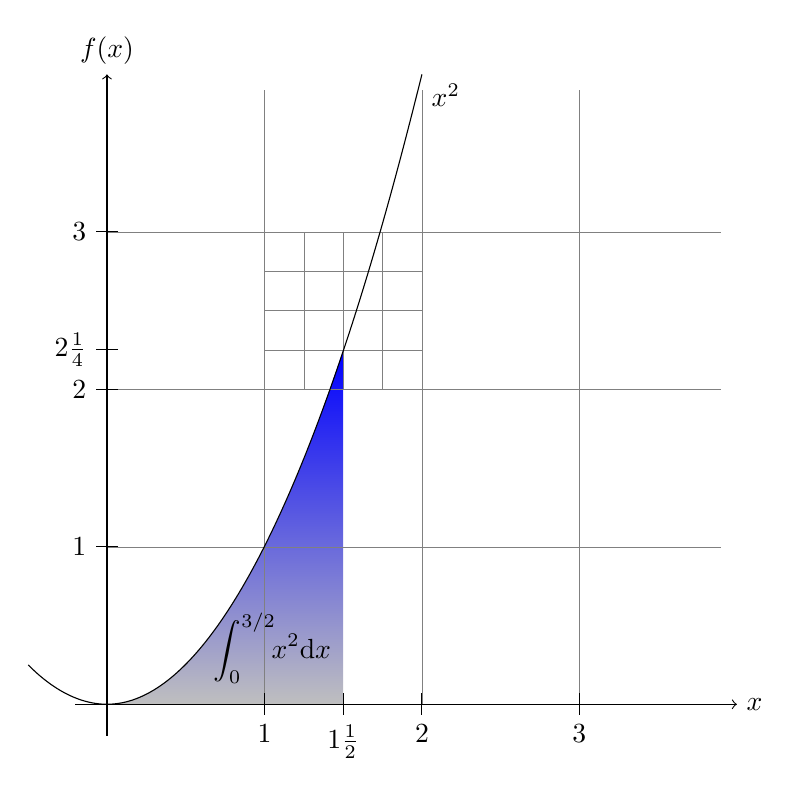
\begin{tikzpicture}[scale=2]
  
  \shade[top color=blue,bottom color=gray!50] (0,0) parabola (1.5,2.25) |- (0,0);
  \draw (1.05cm,2pt) node[above] {$\displaystyle\int_0^{3/2} \!\!x^2\mathrm{d}x$};
  \draw[style=help lines] (0,0) grid (3.9,3.9)
  [step=0.25cm] (1,2) grid +(1,1);
  \draw[->] (-0.2,0) -- (4,0) node[right] {$x$};
  \draw[->] (0,-0.2) -- (0,4) node[above] {$f(x)$};
  \foreach \x/\xtext in {1/1, 1.5/1\frac{1}{2}, 2/2, 3/3}
  \draw[shift={(\x,0)}] (0pt,2pt) -- (0pt,-2pt) node[below] {$\xtext$};
  \foreach \y/\ytext in {1/1, 2/2, 2.25/2\frac{1}{4}, 3/3}
  \draw[shift={(0,\y)}] (2pt,0pt) -- (-2pt,0pt) node[left] {$\ytext$};
  \draw (-.5,.25) parabola bend (0,0) (2,4) node[below right] {$x^2$};
\end{tikzpicture}



\definecolor{wrwrwr}{rgb}{0.3803921568627451,0.3803921568627451,0.3803921568627451}
\definecolor{rvwvcq}{rgb}{0.08235294117647059,0.396078431372549,0.7529411764705882}
\definecolor{sexdts}{rgb}{0.1803921568627451,0.49019607843137253,0.19607843137254902}
\definecolor{cqcqcq}{rgb}{0.7529411764705882,0.7529411764705882,0.7529411764705882}
\begin{tikzpicture}[line cap=round,line join=round,>=triangle 45,x=1cm,y=1cm]
\draw [color=cqcqcq,, xstep=2cm,ystep=2cm] (-7.112751600522956,-8.806454278924885) grid (14.841858065551497,5.0209418697893256);
\draw[->,color=black] (-7.112751600522956,0) -- (14.841858065551497,0);
\foreach \x in {-6,-4,-2,2,4,6,8,10,12,14}
\draw[shift={(\x,0)},color=black] (0pt,2pt) -- (0pt,-2pt) node[below] {\footnotesize $\x$};
\draw[->,color=black] (0,-8.806454278924885) -- (0,5.0209418697893256);
\foreach \y in {-8,-6,-4,-2,2,4}
\draw[shift={(0,\y)},color=black] (2pt,0pt) -- (-2pt,0pt) node[left] {\footnotesize $\y$};
\draw[color=black] (0pt,-10pt) node[right] {\footnotesize $0$};
\clip(-7.112751600522956,-8.806454278924885) rectangle (14.841858065551497,5.0209418697893256);
\fill[line width=2pt,color=rvwvcq,fill=rvwvcq,fill opacity=0.10000000149011612] (0,0) -- (2,0) -- (2,4) -- (1.8343527848910077,3.3648501394373955) -- (1,1) -- (0.5399398893188214,0.29153508407762113) -- cycle;
\draw[line width=2pt,color=sexdts,smooth,samples=100,domain=-7.112751600522956:14.841858065551497] plot(\x,{(\x)^(2)});
\draw[line width=2pt,color=rvwvcq,smooth,samples=100,domain=-7.112751600522956:14.841858065551497] plot(\x,{(\x)+2});
\draw [line width=2pt,color=rvwvcq] (0,0)-- (2,0);
\draw [line width=2pt,color=rvwvcq] (2,0)-- (2,4);
\draw [line width=2pt,color=rvwvcq] (2,4)-- (1.8343527848910077,3.3648501394373955);
\draw [line width=2pt,color=rvwvcq] (1.8343527848910077,3.3648501394373955)-- (1,1);
\draw [line width=2pt,color=rvwvcq] (1,1)-- (0.5399398893188214,0.29153508407762113);
\draw [line width=2pt,color=rvwvcq] (0.5399398893188214,0.29153508407762113)-- (0,0);
\begin{scriptsize}
\draw [fill=wrwrwr] (0,0) circle (2.5pt);
\draw[color=wrwrwr] (0.1683410574956516,0.48974200463096507) node {$A$};
\draw [fill=rvwvcq] (2,0) circle (2.5pt);
\draw[color=rvwvcq] (2.172311513831048,0.48974200463096507) node {$B$};
\draw [fill=wrwrwr] (2,4) circle (2.5pt);
\draw[color=wrwrwr] (2.172311513831048,4.475416578898024) node {$C$};
\draw [fill=rvwvcq] (1.8343527848910077,3.3648501394373955) circle (2.5pt);
\draw[color=rvwvcq] (2.0164471450049617,3.8519591035936798) node {$D$};
\draw [fill=rvwvcq] (1,1) circle (2.5pt);
\draw[color=rvwvcq] (1.1703262856633498,1.469460894394935) node {$E$};
\draw [fill=rvwvcq] (0.5399398893188214,0.29153508407762113) circle (2.5pt);
\draw[color=rvwvcq] (0.7249995175888173,0.7792044038794108) node {$F$};
\end{scriptsize}
\end{tikzpicture}